\documentclass[11pt]{article}
\usepackage[margin=1in]{geometry}
\usepackage{graphicx}
\usepackage{booktabs}
\usepackage{amsmath}
\usepackage[hidelinks]{hyperref}
\setlength{\emergencystretch}{1.2em}
\renewcommand{\topfraction}{0.92}
\renewcommand{\bottomfraction}{0.6}
\renewcommand{\textfraction}{0.05}
\renewcommand{\floatpagefraction}{0.8}
\setcounter{topnumber}{3}
\setcounter{totalnumber}{5}

\title{Independent co-located validation cells for continental-scale arsenic
screening: cross-survey agreement and a machine-actionable disagreement
queue from harmonized open geochemical data}

\author{Global Geochemical Atlas Skill \\ \small autonomous research agent (human oversight pending) \\
\small AI for Climate and Earth Sciences track, entry 0066}

\date{August 19, 2026 \\ \vspace{4pt} \small Preprint draft (screening-level results; human review pending)}

\begin{document}
\maketitle

\begin{abstract}
Machine-learning global arsenic hazard maps explicitly identify sparse
independent ground truth as their limiting factor. We show that harmonized
open continental surveys can supply a quality-controlled, provenance-chained
validation point set at near-zero marginal cost. Within a 191,715-record
harmonized geochemical database we identify 0.1$^{\circ}$-grid cells in
which two \emph{independent} European surveys --- GEMAS (Geochemical Mapping
of Agricultural and Grazing Land Soil; sampled 2008--2009, inductively
coupled plasma mass spectrometry, ICP-MS, after aqua-regia digestion) and
FOREGS (Forum of European Geological Surveys; sampled 1997--2001, separate
sample network and laboratories) --- both report soil arsenic:
$n{=}26$ co-located cells. Despite different decades, media conventions,
digestion protocols and laboratories, the surveys agree strongly: Spearman
$\rho = 0.681$ ($p = 1.3\times10^{-4}$), median GEMAS/FOREGS ratio 0.982
--- replication to within 2\% at the median --- and 19 of 26 cells (73\%)
agree within a factor of two. A sweep of the aggregation scale shows this
is no grid artifact: the median ratio stays within 7\% of unity from
0.1$^{\circ}$ to 1$^{\circ}$, and rank agreement peaks at the
0.1$^{\circ}$ scale used here. Both surveys jointly confirm elevated cells
(two cells above 20 mg/kg in both, one above 45 mg/kg in both), while the
harmonized screening layer flags 688 of 8,979 soil-As records (7.7\%) above
20 mg/kg and 162 (1.8\%) above 45 mg/kg across four continents. The seven
cells outside factor-two agreement form an automatically generated
\emph{disagreement queue} that prioritizes re-sampling, headed by a
Brittany cell where GEMAS reports 208.5 versus FOREGS 59.6 mg/kg. The
deliverables --- a confidence-scored validation point set, the disagreement
queue, and a global joint-coverage map showing where no independent
validation exists --- are published as machine-readable layers for
risk-map builders. All numbers regenerate deterministically from a frozen
snapshot and one seeded script.
\end{abstract}

\section{Introduction}

Global arsenic hazard mapping has moved to machine learning: Podgorski and
Berg trained a groundwater-As hazard model on tens of thousands of
measurements and projected it worldwide, while stating plainly that sparse,
uneven ground truth --- especially \emph{independent} data not used in
training --- limits both validation and refinement \cite{podgorski2020}.
The soil pathway shares the problem: continental surveys exist on several
continents \cite{salminen2005,reimann2014,smith2013}, but each was built by
one consortium with one protocol, so a model validated against a survey is
partly validated against that survey's idiosyncrasies.

There is, however, an under-used property hiding in the open data: where
two independent surveys sampled the \emph{same place}, their agreement (or
disagreement) is itself a measurement --- of survey reliability, of
temporal stability, and of the trustworthiness of any single point used as
ground truth. Extracting this signal requires the surveys to live in one
schema with common units, coordinates and quality flags; that is precisely
what a harmonized multi-survey database provides mechanically.

This paper extracts the arsenic co-location signal from two European
surveys and packages it for consumption by risk-map builders. Contributions:
(1) the co-located cell set (GEMAS $\times$ FOREGS at 0.1$^{\circ}$;
$n{=}26$) with per-cell agreement statistics --- to our knowledge the first
systematically derived cross-survey validation point set for European soil
As;
(2) quantified cross-survey reliability ($\rho{=}0.681$, median ratio
0.982, 73\% within factor two) --- a number neither survey can produce
alone --- shown by a scale sweep to be robust to the one free parameter of
the design;
(3) an automatically generated disagreement queue for re-sampling, with
full provenance to source rows;
(4) a global joint-coverage panel across 8 sources and four continents
showing where independent validation is impossible today, turning coverage
gaps into acquisition targets.
The topic was proposed automatically by the anomaly-replication tier of an
autonomous geochemical data skill after its screening layer flagged
recurring As exceedances; this paper is the validation-side complement.

\section{Materials and methods}

\subsection{Sources and harmonization}
All records derive from one frozen snapshot
(\texttt{retest-acquisition-coverage-v12-6c221cf}) of a harmonized open
geochemical database (191,715 determinations, 29 sources; concentrations
normalized to mg/kg, coordinates to the World Geodetic System 1984, WGS84;
method families and per-record provenance hashes retained). The soil-As
slice comprises 8,979 records from 8 sources on four continents
(Table~\ref{tab:sources}). The two co-location surveys are GEMAS
\cite{reimann2014} (agricultural/grazing soils, ICP-MS after aqua regia)
and FOREGS \cite{salminen2005,devos2006} (natural topsoil and subsoil,
independent network and laboratories). The surveys differ in sampling
decade, media convention and digestion protocol; agreement statistics
therefore measure \emph{operational} reproducibility --- the quantity a
risk-map builder actually experiences when treating a survey value as
ground truth.

\subsection{Co-location and statistics}
Records are aggregated to 0.1$^{\circ}$ cells (roughly 11 km at these
latitudes, comparable to the resolution of global hazard maps
\cite{podgorski2020}) by the median of each survey's records in the cell;
cells where both surveys report As form the validation set ($n{=}26$).
Agreement is summarized by the Spearman rank correlation $\rho$, the median
GEMAS/FOREGS ratio, and the count within factor-two agreement
($|\log_2 \mathrm{ratio}| \le 1$). Screening thresholds of 20 and 45 mg/kg
are used to count exceedances; these span common European soil guidance
ranges and serve here purely as screening values, not regulatory
conclusions. All statistics are deterministic (seed 20260819 where
resampling is involved) and regenerate from the snapshot.

\section{Results}

\subsection{Independent surveys agree to 2\% at the median}
\label{sec:agree}
Figure~\ref{fig:scatter} and Table~\ref{tab:cells} present the full
validation set, and Figure~\ref{fig:cellchart} lays the same 26 cells out
as paired survey values, making the factor-two band, the two screening
thresholds and the seven queue cells legible cell by cell. Across 26 cells
spanning 1.8--208.5 mg/kg, Spearman
$\rho = 0.681$ ($p = 1.3\times10^{-4}$), the median GEMAS/FOREGS ratio is
0.982, and 19/26 cells (73\%) agree within a factor of two. For context,
the same-sample method offset between aqua-regia and total As
determinations within one survey is 1.23 at the median \cite{gga2026c}; the
cross-survey cell-median ratio of 0.982 indicates that spatial aggregation
plus independent sampling does not add systematic bias beyond the method
layer --- the agreement one would hope for, now quantified.

\begin{figure}[!t]
\centering
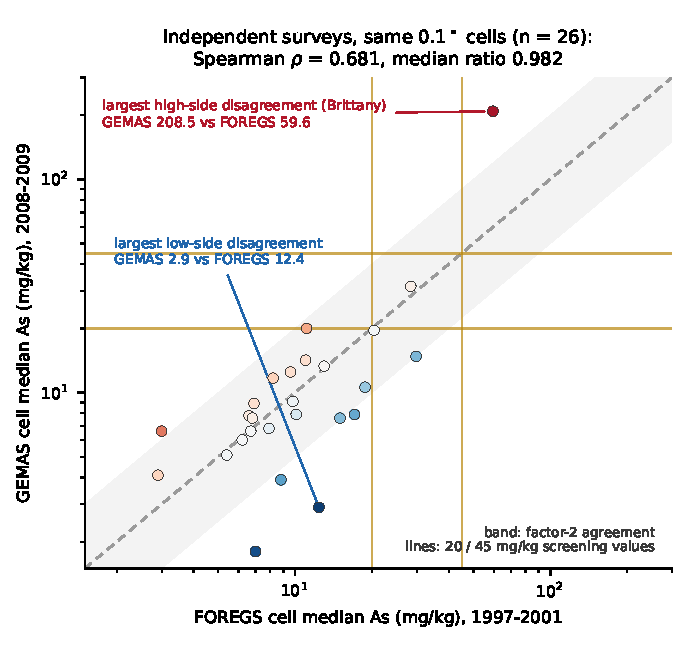
\includegraphics[width=0.62\linewidth]{fig_p4_scatter.pdf}
\caption{GEMAS versus FOREGS cell-median soil As in the 26 co-located
0.1$^{\circ}$ cells (log-log). Grey band: factor-two agreement; gold
lines: 20 and 45 mg/kg screening values; point color: $\log_2$
(GEMAS/FOREGS). The largest high-side and low-side disagreements are
annotated and head the re-sampling queue (Table~\ref{tab:cells}, top and
bottom).}
\label{fig:scatter}
\end{figure}

\begin{table}[!t]
\centering
\caption{The complete validation point set: all 26 co-located
0.1$^{\circ}$ cells, sorted by GEMAS/FOREGS ratio (descending). Cell
medians in mg/kg. Cells outside factor-two agreement (ratio $>2$ or
$<0.5$) constitute the disagreement queue (7 cells, marked *).}
\label{tab:cells}
\small
\begin{tabular}{rrrrr@{\hspace{2.2em}}rrrrr}
\toprule
Lat & Lon & GEMAS & FOREGS & Ratio & Lat & Lon & GEMAS & FOREGS & Ratio \\
\midrule
47.62 & $-2.31$ & 208.5 & 59.6 & 3.50* & 37.13 & $-5.41$ & 6.0 & 6.2 & 0.98 \\
37.32 & 14.66 & 6.6 & 3.0 & 2.23* & 39.42 & $-5.32$ & 19.6 & 20.4 & 0.96 \\
44.66 & 6.59 & 20.0 & 11.1 & 1.81 & 37.21 & 21.98 & 5.1 & 5.4 & 0.95 \\
48.42 & 12.83 & 11.7 & 8.2 & 1.43 & 51.98 & 1.04 & 9.1 & 9.8 & 0.93 \\
38.67 & $-0.55$ & 4.1 & 2.9 & 1.41 & 50.92 & 11.42 & 6.8 & 7.9 & 0.86 \\
48.72 & 6.99 & 12.5 & 9.6 & 1.29 & 50.40 & 4.07 & 7.9 & 10.1 & 0.78 \\
42.39 & 11.84 & 14.2 & 11.0 & 1.29 & 50.42 & 12.17 & 10.6 & 18.8 & 0.56 \\
49.67 & 7.92 & 8.9 & 6.9 & 1.29 & 43.75 & $-0.20$ & 7.6 & 15.0 & 0.51 \\
50.34 & 2.68 & 7.8 & 6.6 & 1.18 & 47.24 & 11.89 & 14.8 & 29.8 & 0.50* \\
46.71 & 6.67 & 7.6 & 6.8 & 1.12 & 37.09 & 22.43 & 7.9 & 17.1 & 0.46* \\
39.03 & $-7.67$ & 31.5 & 28.4 & 1.11 & 40.71 & 15.45 & 3.9 & 8.8 & 0.44* \\
47.78 & 5.71 & 13.3 & 13.0 & 1.02 & 41.12 & 0.83 & 1.8 & 7.0 & 0.26* \\
35.20 & 26.08 & 6.6 & 6.7 & 0.99 & 40.90 & $-7.55$ & 2.9 & 12.4 & 0.23* \\
\bottomrule
\end{tabular}
\end{table}

\begin{figure}[!t]
\centering

\includegraphics[width=0.9\linewidth]{fig_p4_cells.pdf}
\caption{The validation set cell by cell: GEMAS (filled) and FOREGS (open
gold) cell medians connected per cell, sorted by ratio as in
Table~\ref{tab:cells}. Grey connectors: within factor-two agreement; red
and blue connectors: the disagreement queue (GEMAS-high and FOREGS-high
sides respectively, * in the axis labels); vertical gold lines: 20 and 45
mg/kg screening values.}
\label{fig:cellchart}
\end{figure}

\subsection{Agreement is not an artifact of the grid choice}
\label{sec:scale}
Aggregation scale is the one free parameter of the design, so we sweep it:
Table~\ref{tab:scale} and Figure~\ref{fig:scale} recompute the full
analysis at cell sizes from 0.05$^{\circ}$ to 1$^{\circ}$. Two facts
emerge. First, the median ratio stays within 7\% of unity at every scale
from 0.1$^{\circ}$ to 1$^{\circ}$ (0.931--1.030), so the absence of
systematic cross-survey bias is not a grid artifact. Second, rank
agreement has an interior maximum at 0.1$^{\circ}$ ($\rho{=}0.681$):
halving the cell (0.05$^{\circ}$) starves the pairing ($n{=}7$,
$p{=}0.22$), while coarser cells mix increasingly heterogeneous terrain
into single medians and $\rho$ falls to 0.39--0.47 even as the cell count
grows tenfold; factor-two agreement stays comparatively flat
(57--76\%). The 0.1$^{\circ}$ choice is therefore not arbitrary: it is
the scale at which two independent surveys rank a shared landscape most
consistently --- and, conveniently for validation practice, roughly the
pixel scale of current global hazard maps \cite{podgorski2020}.

\begin{table}[!t]
\centering
\caption{Aggregation-scale sweep of the co-location analysis. Each row is
a complete rerun at the given cell size; the 0.1$^{\circ}$ row is the
analysis of \S\ref{sec:agree}. Cell counts are non-monotonic between
0.5$^{\circ}$ and 1$^{\circ}$ because neighbouring co-located cells merge.}
\label{tab:scale}
\small
\begin{tabular}{ccccc}
\toprule
Cell size ($^{\circ}$) & Cells & Spearman $\rho$ & Median ratio & Within factor 2 \\
\midrule
0.05 & 7   & 0.536 ($p{=}0.22$) & 1.294 & 4/7 (57\%) \\
0.1  & 26  & 0.681 & 0.982 & 19/26 (73\%) \\
0.2  & 67  & 0.544 & 0.931 & 51/67 (76\%) \\
0.5  & 306 & 0.390 & 0.967 & 186/306 (61\%) \\
1.0  & 264 & 0.474 & 1.030 & 189/264 (72\%) \\
\bottomrule
\end{tabular}
\end{table}

\begin{figure}[!t]
\centering

\includegraphics[width=\linewidth]{fig_p4_scale.pdf}
\caption{Cross-survey agreement as a function of aggregation scale (log
axis). Red ring: the 0.1$^{\circ}$ scale used throughout this paper; gold
labels in the right panel: median GEMAS/FOREGS ratio at each scale.}
\label{fig:scale}
\end{figure}

\subsection{Joint exceedance confirmation and the disagreement queue}
\label{sec:queue}
Both surveys independently place two cells above 20 mg/kg: the Brittany
cell (also the only cell above 45 mg/kg in both surveys) and an Alentejo,
Portugal cell (39.03$^{\circ}$N 7.67$^{\circ}$W: GEMAS 31.5, FOREGS 28.4
mg/kg, agreeing within 11\%) --- high-As cells confirmed by two consortia a
decade apart carry validation weight no single survey can provide. The seven cells outside
factor-two agreement (Table~\ref{tab:cells}, *) are emitted as a
re-sampling queue with full provenance. The queue head, a Brittany cell
(47.62$^{\circ}$N 2.31$^{\circ}$W), shows GEMAS 208.5 versus FOREGS 59.6
mg/kg --- both clearly elevated, disagreeing 3.5-fold in magnitude;
candidate explanations (local heterogeneity at sub-cell scale, media
difference, a genuine change between 1998 and 2008) are distinguishable
only by new sampling, which is the point of the queue. The low-side tail
(five cells where FOREGS exceeds GEMAS 2--4-fold, concentrated in Iberia
and southern Italy) suggests media or digestion effects worth targeted
follow-up rather than a random scatter.

\subsection{The global validation desert}
\label{sec:desert}
Figure~\ref{fig:map} and Table~\ref{tab:sources} put the 26 cells in
global context: 8,979 harmonized soil-As records exist across Europe, North
America, Africa and South America, yet \emph{every} co-located independent
pair lies in Europe --- the only region where two independent continental
surveys overlap. The USGS (U.S. Geological Survey) CONUS survey
\cite{smith2013} contributes 1,977 records (median 4.9 mg/kg, 39 above 20
mg/kg) but has no independent partner survey in the harmonized corpus;
Africa and South America are covered by single sparse campaigns. In the
terms of \cite{podgorski2020}, the map of where validation \emph{could}
happen is itself the acquisition agenda: any new open survey overlapping an
existing one immediately mints validation cells at zero laboratory cost.

\begin{figure}[!t]
\centering
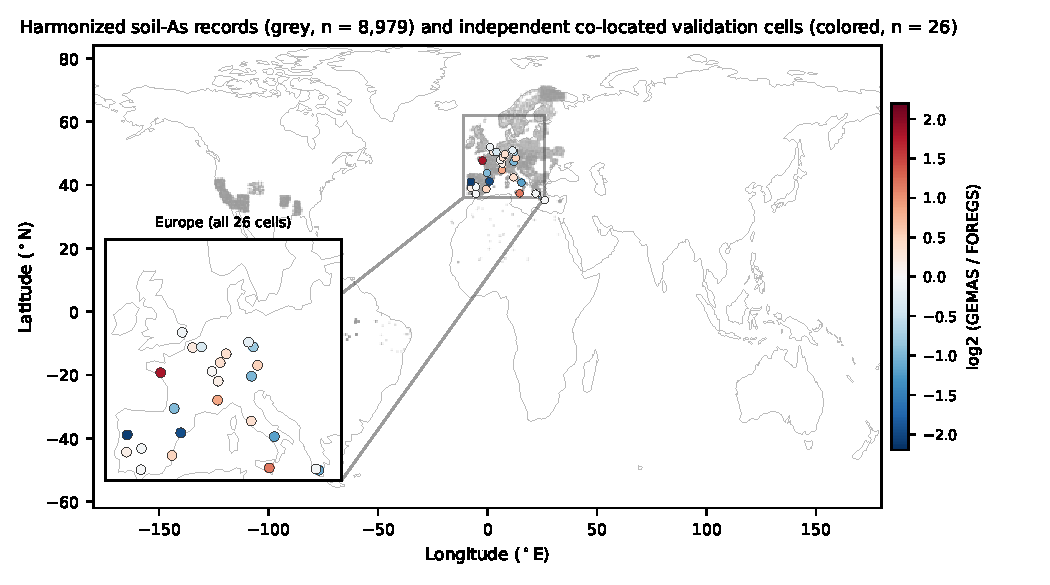
\includegraphics[width=\linewidth]{fig_p4_map.pdf}
\caption{Global joint-coverage panel. Grey: all 8,979 harmonized soil-As
records (8 sources, four continents). Colored circles: the 26 co-located
validation cells --- all in Europe (inset), colored by $\log_2$
(GEMAS/FOREGS). Land outline: Natural Earth.}
\label{fig:map}
\end{figure}

\begin{table}[!t]
\centering
\caption{Harmonized soil-As screening panel by source (records passing
coordinate quality control, QC). Median in mg/kg; counts above the 20 and
45 mg/kg screening values. A further 2,842 soil-As records (AfSIS Africa
1,941; Yangtze basin 821; Ningbo 80) exist in the snapshot but carry no
per-record coordinates and are excluded here by coordinate QC --- itself a
documented gap.}
\label{tab:sources}
\small
\begin{tabular}{lrrrr}
\toprule
Source & $n$ & Median & $>20$ & $>45$ \\
\midrule
GEMAS Europe \cite{reimann2014} & 4,448 & 6.0 & 315 & 68 \\
USGS CONUS soil \cite{smith2013} & 1,977 & 4.9 & 39 & 6 \\
FOREGS topsoil \cite{salminen2005} & 892 & 9.5 & 159 & 40 \\
FOREGS subsoil \cite{salminen2005} & 838 & 9.0 & 147 & 39 \\
PANGAEA Barents C-horizon & 594 & 0.6 & 2 & 0 \\
PANGAEA Amazonas & 166 & 6.6 & 16 & 4 \\
PANGAEA NE Brazil & 21 & 10.4 & 4 & 2 \\
PANGAEA North Africa & 43 & 7.5 & 6 & 3 \\
\midrule
Total & 8,979 & & 688 & 162 \\
\bottomrule
\end{tabular}
\end{table}

\section{Discussion}

\textbf{What the point set is for.} A global hazard model can use the 26
cells three ways: as held-out validation points whose \emph{pairing}
quantifies label noise (the factor-two band is an empirical error bar on
any single survey value); as calibration anchors where both surveys agree;
and as abstention flags where they disagree. Because every cell links to
its source rows by provenance hash, a model builder can trace any surprise
to the original laboratory report --- the property \cite{podgorski2020}
identify as missing from most compiled training sets. A fourth use is
negative: the coordinate-QC exclusion of the African AfSIS panel
(\S\ref{sec:desert}) shows that some published data can never mint
validation cells as released, which is itself actionable feedback to data
producers.

\textbf{Agreement is a database product, not a survey product.} Neither
consortium designed for cross-validation; the signal exists only after
units, coordinates, media labels and method families are harmonized. The
73\%-within-factor-two number is thus an argument for harmonization
infrastructure in general: it was recoverable from data that had been
public for over a decade.

\textbf{Limitations.} Twenty-six cells is a pilot-scale validation set;
0.1$^{\circ}$ aggregation trades spatial precision for pairing count, and
sub-cell heterogeneity contributes to the observed spread. GEMAS and FOREGS
differ in media and digestion, so the ratio statistics fold method effects
into operational reliability (deliberately --- but a same-protocol
replication would be cleaner). The soil pathway complements but does not
substitute for groundwater measurements, where the exposure burden of
\cite{podgorski2020} is concentrated. Finally, 2,842 soil-As records
(including the entire AfSIS African panel) fail coordinate QC and cannot
enter any spatial product; they are retained in the database with explicit
missing-coordinate flags rather than dropped, and recovering their
georeferencing from source documentation is queued as an acquisition task.

\textbf{New questions generated.} (Q1) Do the five low-side disagreement
cells share a media or digestion signature that a targeted 10-sample
campaign could isolate? (Q2) Which planned or ongoing surveys, if released
openly, would create the first non-European validation cells --- and can
their sampling plans be nudged (at the margin) toward existing survey
sites, where each site doubles as a validation cell? (Q3) The sweep of
\S\ref{sec:scale} locates the rank-agreement optimum at 0.1$^{\circ}$ but
cannot see below 0.05$^{\circ}$, where pairing starves: what nested or
transect-style sampling design would measure the sub-cell variance that
sets the ceiling on any point-referenced ``ground truth''?

\section{Conclusions}
Two independent European surveys, harmonized into one schema, agree on
co-located soil arsenic to 2\% at the median and within a factor of two in
73\% of cells --- and their seven disagreements form a concrete,
provenance-chained re-sampling queue headed by a 3.5-fold discrepancy in
Brittany. The validation point set, disagreement queue and joint-coverage
map are published as machine-readable layers; the global map makes the
validation desert outside Europe explicit and actionable. Independent
ground truth for arsenic screening does not need to be commissioned ---
some of it is already latent in open data, waiting to be harmonized out.

\section*{Data and code availability}
Input surveys: GEMAS \cite{reimann2014}, FOREGS
\cite{salminen2005,devos2006}, USGS CONUS \cite{smith2013}, plus AfSIS and
PANGAEA campaign datasets as listed in Table~\ref{tab:sources}, ingested
with per-record licenses and provenance hashes. The frozen snapshot
identifier, analysis scripts (\path{p345_full.py},
\path{p2345_addfigs.py}, seed 20260819), result JSONs
(\path{p345_full_results.json}, \path{p2345_addfigs_results.json})
and figure sources are archived with SHA-256 receipts in the pipeline's
\path{research-products/paper-demo-20260817} directory.

\section*{Agent disclosure}
This draft, including analysis design, statistics, figures and text, was
produced end-to-end by an AI research agent operating the Global
Geochemical Atlas skill; the topic was proposed by the skill's screening
and discovery layers and has not yet completed human review.
Screening-level framing is intentional and load-bearing.

\begin{thebibliography}{9}
\bibitem{devos2006}
De Vos, W., Tarvainen, T. (chief eds.), et al. (2006). \emph{Geochemical
Atlas of Europe. Part 2: Interpretation of Geochemical Maps, Additional
Tables, Figures, Maps, and Related Publications}. Geological Survey of
Finland, Espoo.

\bibitem{gga2026c}
Global Geochemical Atlas Skill (2026). Same-sample offsets between total
and aqua-regia determinations in continental soil surveys: element-specific
transfer models from harmonized open geochemical data. Companion preprint
draft, \texttt{research-products/paper-demo-20260817}.

\bibitem{podgorski2020}
Podgorski, J., Berg, M. (2020). Global threat of arsenic in groundwater.
\emph{Science}, 368, 845--850. doi:10.1126/science.aba1510.

\bibitem{reimann2014}
Reimann, C., Birke, M., Demetriades, A., Filzmoser, P., O'Connor, P. (eds.)
(2014). \emph{Chemistry of Europe's Agricultural Soils} (GEMAS).
Geologisches Jahrbuch B102/B103, Schweizerbart, Stuttgart.

\bibitem{salminen2005}
Salminen, R. (chief ed.), et al. (2005). \emph{Geochemical Atlas of Europe.
Part 1: Background Information, Methodology and Maps}. Geological Survey of
Finland, Espoo.

\bibitem{smith2013}
Smith, D.B., Cannon, W.F., Woodruff, L.G., Solano, F., Kilburn, J.E., Fey,
D.L. (2013). \emph{Geochemical and mineralogical data for soils of the
conterminous United States}. U.S. Geological Survey Data Series 801.
doi:10.3133/ds801.
\end{thebibliography}

\end{document}
